
\documentclass[runningheads]{llncs}
\usepackage[paperheight=295mm,paperwidth=210mm]{geometry}
\usepackage{graphicx}
\usepackage{kotex}
\usepackage[dvipsnames]{xcolor}
\usepackage{fancyvrb}
\usepackage{listings}
\usepackage{indentfirst}
\usepackage{tabularx}
\usepackage{underscore}
\usepackage{multicol}
\usepackage[square,sort,comma,super]{natbib}
\usepackage{inconsolata} % Inconsolata
\usepackage{mathptmx} % Times New Roman
\usepackage[cache=false]{minted}
\graphicspath{ {./images/} }
\lstset{basicstyle=\footnotesize\ttfamily,breaklines=true}
\renewcommand{\bibname}{참고문헌}
\setlength{\parindent}{1em}
\setlength{\parskip}{1em}
\linespread{1.2}
{\renewcommand{\arraystretch}{1.5}%
\setlength{\tabcolsep}{0.5em}%
\newenvironment{Figure}
  {\par\medskip\noindent\minipage{\linewidth}}
  {\endminipage\par\medskip}
	
\begin{document}

\title{CSE3013 (컴퓨터공학 설계 및 실험 I) \space \newline WEB-2 예비 보고서}
\author{서강대학교 컴퓨터공학과 박수현 (20181634)}
\institute{서강대학교 컴퓨터공학과}
\maketitle

\section{목적}
PHP의 기본 문법과 실험을 수행할 수 있는 배경 지식을 공부한다.

\section{문제 풀이}

\subsection{PHP 환경변수 값 알아보기}

\begin{tabular}{ l | l }
	\hline
	변수 이름 & 값 \\
	\hline
	\texttt{\$\_SERVER["PHP\_SELF"]} & 현재 실행 중인 스크립트의 파일명 \\
	\texttt{\$\_SERVER["SERVER\_NAME"]} & 호스트 서버 이름 \\
	\texttt{\$\_SERVER["SCRIPT\_FILENAME"]} & 현재 실행되고 있는 스크립트의 절대 주소 \\
	\texttt{\$\_SERVER["SERVER\_SOFTWARE"]} & 서버 증명 문자열 \\
	\texttt{\$\_SERVER["SERVER\_ADDR"]} & 호스트 서버 IP \\
	\texttt{\$\_SERVER["SERVER\_PORT"]} & 커뮤니케이션을 위해 사용되는 포트 \\
	\texttt{\$\_SERVER["SERVER\_PROTOCOL"]} & 프로토콜의 이름과 버전 \\
	\hline
\end{tabular}

\newpage
\subsection{PHP 프로그래밍의 기초 문법}

\begin{multicols}{2}
	\begin{Figure}
		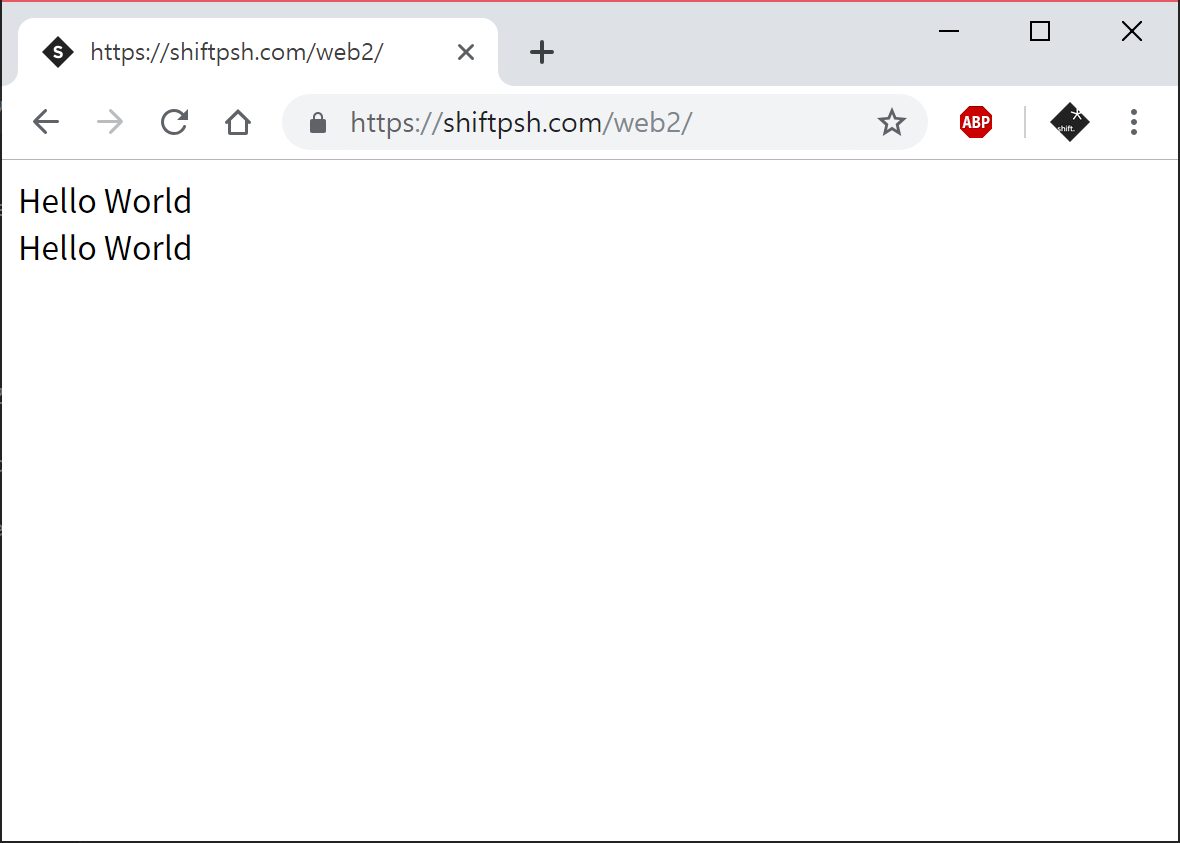
\includegraphics[width=\linewidth]{preview-3-1}
		\label{fig:preview-3-1}
	\end{Figure}
	\columnbreak
	\begin{minipage}{\columnwidth}
		\inputminted[xleftmargin=\parindent,linenos]{php}{inc-sources/source-3-1.php}
	\end{minipage}
\end{multicols}

\subsection{PHP 프로그래밍의 함수}

\begin{multicols}{2}
	\begin{Figure}
		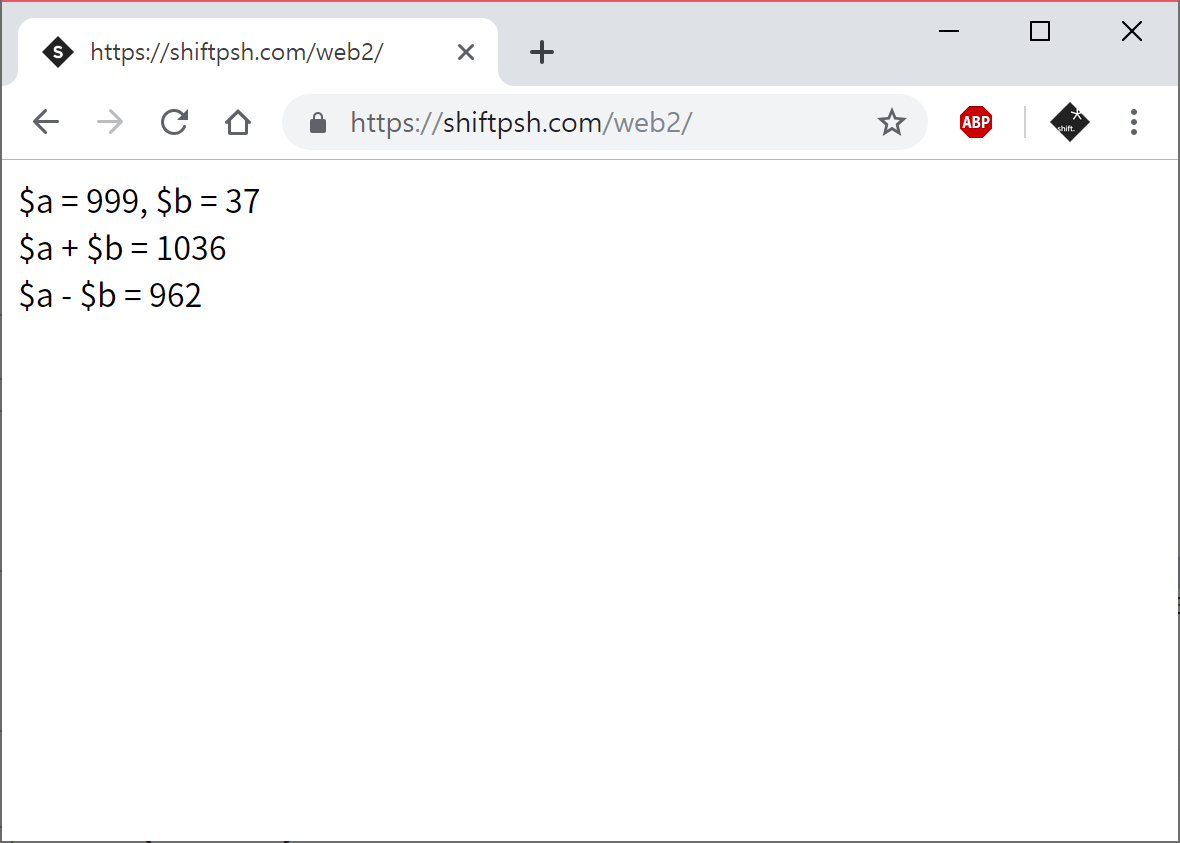
\includegraphics[width=\linewidth]{preview-3-2}
		\label{fig:preview-3-2}
	\end{Figure}
	\columnbreak
	\begin{minipage}{\columnwidth}
		\inputminted[xleftmargin=\parindent,linenos]{php}{inc-sources/source-3-2.php}
	\end{minipage}
\end{multicols}

\subsection{PHP 프로그래밍의 응용}

\begin{Figure}
	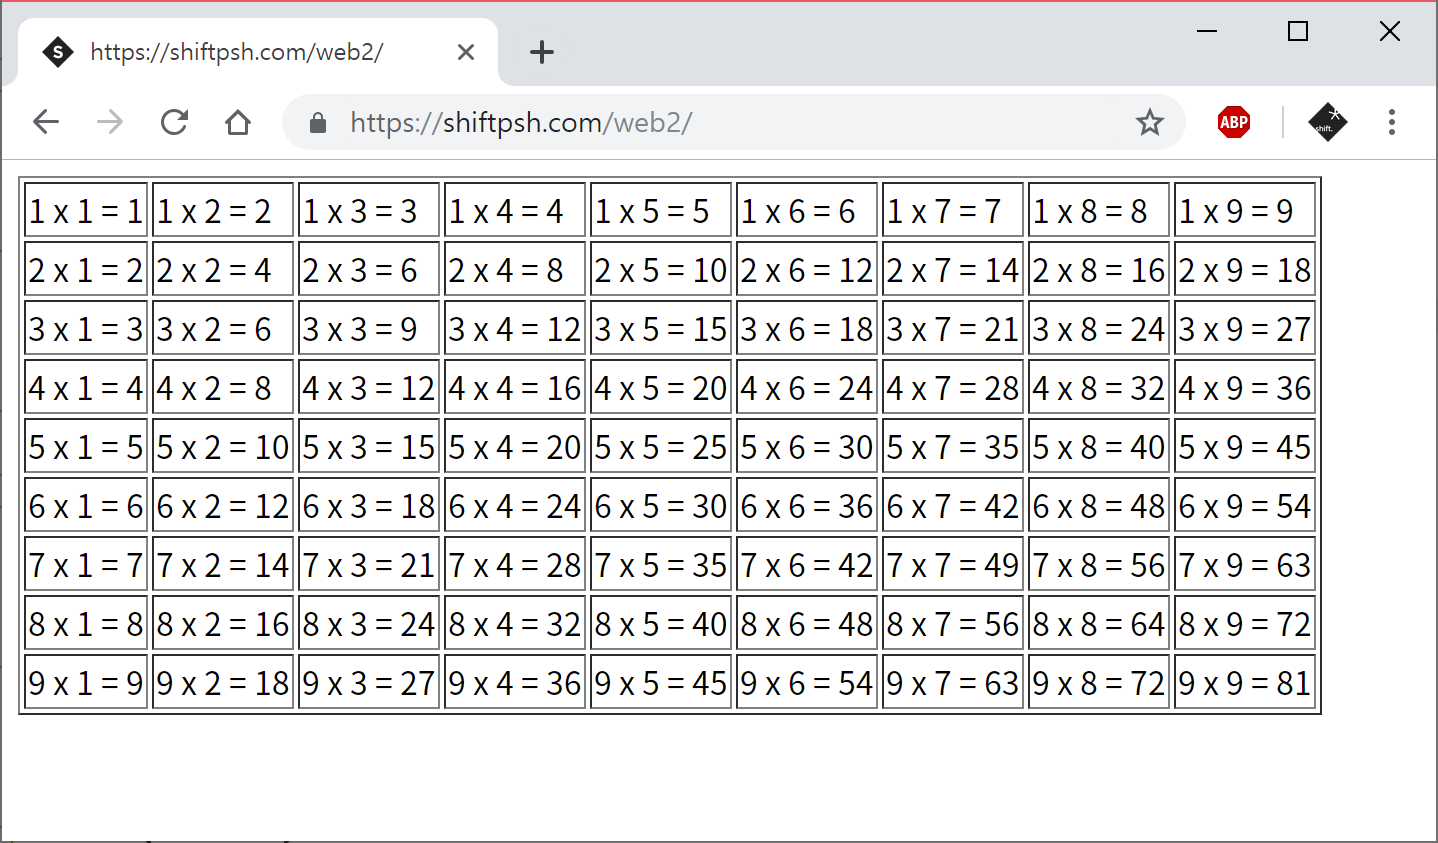
\includegraphics[width=\linewidth]{preview-3-3}
	\label{fig:preview-3-3}
\end{Figure}

\inputminted[xleftmargin=\parindent,linenos]{php}{inc-sources/source-3-3.php}
  
\end{document}
